\documentclass[tikz,border=2pt]{standalone}
\usepackage{amsmath,amssymb}
\usepackage{pgfplots}
\pgfplotsset{compat=1.18}
\usetikzlibrary{calc}

\begin{document}
% F_X(x) = P(X <= x): a right-continuous staircase for a discrete variable (jumps = pmf), a
% smooth S-curve for a continuous one; always nondecreasing from 0 to 1.
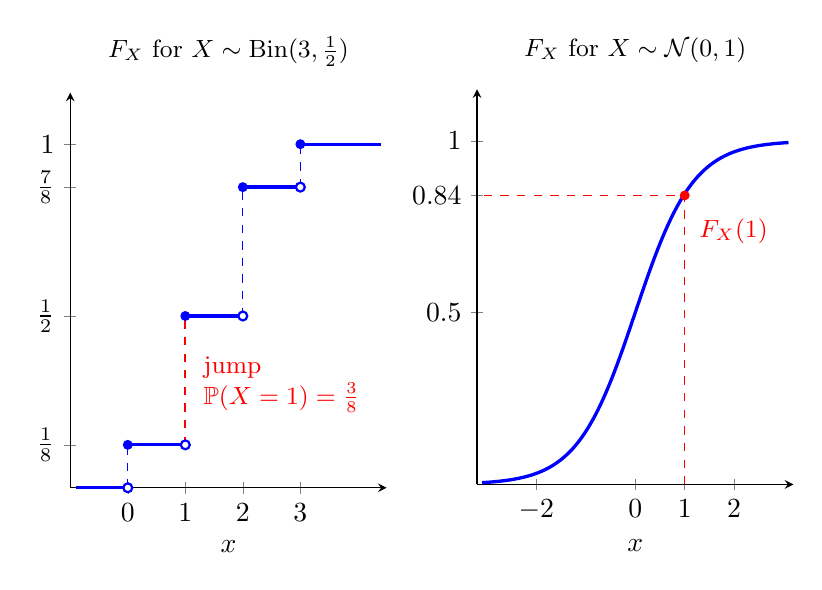
\begin{tikzpicture}
	\begin{axis}[
		name=p1, axis lines=left, xmin=-1, xmax=4.5, ymin=0, ymax=1.15,
		xtick={0,1,2,3}, ytick={0.125,0.5,0.875,1}, yticklabels={$\tfrac18$,$\tfrac12$,$\tfrac78$,$1$},
		xlabel={$x$},
		width=5.6cm, height=6.6cm, clip=false, title={$F_X$ for $X\sim\operatorname{Bin}(3,\tfrac12)$}, title style={font=\small}
		]
		\draw[blue, very thick] (axis cs:-0.9,0) -- (axis cs:0,0);
		\draw[blue, very thick] (axis cs:0,0.125) -- (axis cs:1,0.125);
		\draw[blue, very thick] (axis cs:1,0.5) -- (axis cs:2,0.5);
		\draw[blue, very thick] (axis cs:2,0.875) -- (axis cs:3,0.875);
		\draw[blue, very thick] (axis cs:3,1) -- (axis cs:4.4,1);
		\draw[blue, dashed] (axis cs:0,0) -- (axis cs:0,0.125);
		\draw[red, thick, dashed] (axis cs:1,0.125) -- (axis cs:1,0.5);
		\draw[blue, dashed] (axis cs:2,0.5) -- (axis cs:2,0.875);
		\draw[blue, dashed] (axis cs:3,0.875) -- (axis cs:3,1);
		\draw[blue, fill=white, thick] (axis cs:0,0) circle (1.6pt);
		\draw[blue, fill=white, thick] (axis cs:1,0.125) circle (1.6pt);
		\draw[blue, fill=white, thick] (axis cs:2,0.5) circle (1.6pt);
		\draw[blue, fill=white, thick] (axis cs:3,0.875) circle (1.6pt);
		\fill[blue] (axis cs:0,0.125) circle (1.8pt);
		\fill[blue] (axis cs:1,0.5) circle (1.8pt);
		\fill[blue] (axis cs:2,0.875) circle (1.8pt);
		\fill[blue] (axis cs:3,1) circle (1.8pt);
		\node[red, font=\small, anchor=west, align=left] at (axis cs:1.15,0.3) {jump\\ $\mathbb{P}(X=1)=\tfrac38$};
	\end{axis}
	\begin{axis}[
		name=p2, at={(p1.outer east)}, anchor=outer west, xshift=2mm,
		axis lines=left, xmin=-3.2, xmax=3.2, ymin=0, ymax=1.15,
		xtick={-2,0,1,2}, ytick={0.5,0.841,1}, yticklabels={$0.5$,$0.84$,$1$},
		xlabel={$x$},
		samples=120, smooth, width=5.6cm, height=6.6cm, clip=false, title={$F_X$ for $X\sim\mathcal{N}(0,1)$}, title style={font=\small}
		]
		\addplot[blue, very thick, domain=-3.1:3.1] {1/(1+exp(-1.702*x))};
		\draw[red, dashed] (axis cs:1,0) -- (axis cs:1,0.841) -- (axis cs:-3.2,0.841);
		\fill[red] (axis cs:1,0.841) circle (1.8pt);
		\node[red, font=\small, anchor=north west] at (axis cs:1.1,0.8) {$F_X(1)$};
	\end{axis}
	
\end{tikzpicture}
\end{document}
